\documentclass[12pt,a4paper,english]{article}
\usepackage{graphicx}
\usepackage[english]{babel}
\usepackage[utf8]{inputenc}
%\usepackage{listings}
\usepackage{multirow}
\usepackage{epstopdf}
\usepackage{amsmath}
\usepackage{amssymb}
\usepackage{mathpazo}
\usepackage{csquotes}
\usepackage{siunitx}
\usepackage{tikz}
\usepackage{booktabs}
\usepackage{parskip}
\graphicspath{{./fig/}}

\setlength{\hoffset}{-1in} \setlength{\textwidth}{18cm}
\setlength{\oddsidemargin}{1.5cm}
\setlength{\evensidemargin}{1.5cm}
\setlength{\marginparsep}{0.7em}
\setlength{\marginparwidth}{0.5cm}

\setlength{\voffset}{-1.9in}
\setlength{\headheight}{12pt}
\setlength{\topmargin}{2.6cm}
   \addtolength{\topmargin}{-\headheight}
\setlength{\headsep}{3.5cm}
   \addtolength{\headsep}{-\topmargin}
   \addtolength{\headsep}{-\headheight}
\setlength{\textheight}{27cm}

%% How should floats be treated?
\setlength{\floatsep}{12 pt plus 0 pt minus 8 pt}
\setlength{\textfloatsep}{12 pt plus 0pt minus 8 pt}
\setlength{\intextsep}{12 pt plus 0pt minus 8 pt}

\tolerance2000
\emergencystretch20pt

%% Text appearence
% English text
\newcommand{\eg}[1]%
  {\selectlanguage{english}\textit{#1}\selectlanguage{austrian}}

\newcommand{\filename}[1]
  {\begin{small}\texttt{#1}\end{small}}

\newcommand\IFT{\unitlength1mm\begin{picture}(10,2) \put (1,1)
{\circle{1.7}} \put(2,1){\line(1,0){5}} \put(8,1)
{\circle*{1.7}}\end{picture}}
\newcommand\FT{\unitlength1mm\begin{picture}(10,2) \put (1,1)
{\circle*{1.7}} \put(2,1){\line(1,0){5}} \put(8,1)
{\circle{1.7}}\end{picture}}

% A box for multiple choice problems
\newcommand{\choicebox}{\fbox{\rule{0pt}{0.5ex}\rule{0.5ex}{0pt}}}

\newenvironment{truefalse}%
  {\bigskip\par\noindent\makebox[1cm][c]{true}\hspace{3mm}\makebox[1cm][c]{false}
   \begin{list}%
   {\makebox[1cm][c]{\choicebox}\hspace{3mm}\makebox[1cm][c]{\choicebox}}%
   {\setlength{\labelwidth}{2.31 cm}\setlength{\labelsep}{3mm}
    \setlength{\leftmargin}{2.61 cm}\setlength{\listparindent}{0pt}
    \setlength{\itemindent}{0pt}}%
  }
  {\end{list}}

\newcounter{theexercise}\setcounter{theexercise}{1}
\newenvironment{exercise}[1]%
  {\bigskip\par\noindent\begin{nopagebreak}
   \textsf{\textbf{Exercise \arabic{theexercise}}}\quad
      \textsf{\textit{#1}}\\*[1ex]%
\stepcounter{theexercise}\hspace{2ex}\end{nopagebreak}}
  {\par\pagebreak[2]}

\renewcommand{\labelenumi}{\alph{enumi})}
\renewcommand{\labelenumii}{\arabic{enumii})}

% A box to tick for everything which has to done
\newcommand{\abgabe}{\marginpar{$\Box$}}
% Margin paragraphs on the left side
\reversemarginpar

% Language for listings
%\lstset{language=Vhdl,
%  basicstyle=\small\tt,
 % keywordstyle=\tt\bf,
 % commentstyle=\sl}

% No indention
\setlength{\parindent}{0.0cm}
% Don't number sections
\setcounter{secnumdepth}{0}

\DeclareMathOperator{\atantwo}{atan2}

%% Beginning of the text

\begin{document}
\selectlanguage{english}
\pagestyle{plain}

\thispagestyle{empty}
\noindent
\begin{minipage}[b][4cm]{1.0\textwidth}
    \begin{center}
        \begin{bf}
            \begin{large}
                Digital Signal Processing 2024S -- Assignment 4
            \end{large} \\
            \vspace{0.3cm}
            \begin{Large}
                Reconstruction, DFT, FFT, STFT
            \end{Large} \\
            \vspace{0.3cm}
        \end{bf}
        \begin{large}
            Group 52\\
            Laurenz Weixlbaumer, k11804751\\
            Jannik Jungmann, k12103135\\
        \end{large}
    \end{center}
\end{minipage}

\noindent \rule[0.8em]{\textwidth}{0.12mm}\\[-0.5em]

\begin{exercise}{Reconstruction}
    \begin{enumerate}
        \item See Figures \ref{fig:ex1_1} and \ref{fig:ex1_2}.

              \begin{figure}[ht]
                  \centering
                  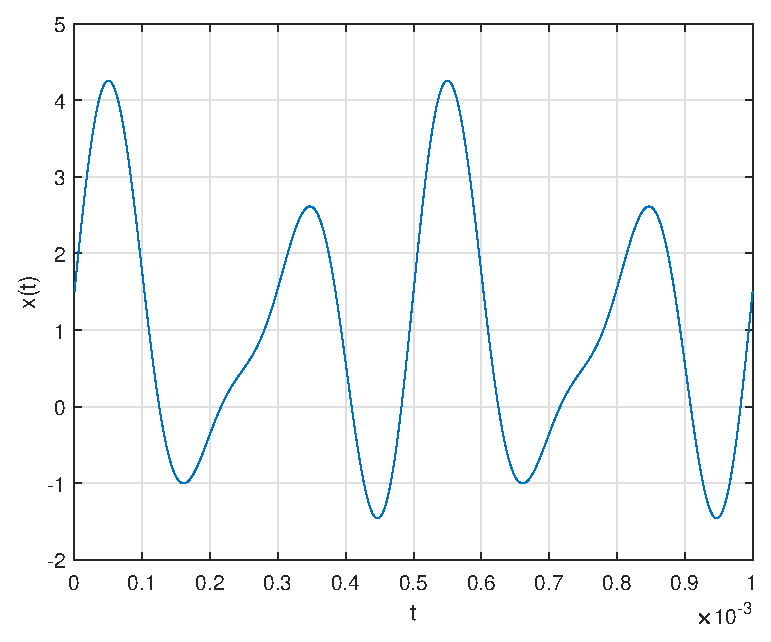
\includegraphics{fig/ex1_1.eps}
                  \caption{Plot of the analog signal $x(t)$}
                  \label{fig:ex1_1}
              \end{figure}

              \begin{figure}[ht]
                  \centering
                  \begin{tikzpicture}
                      \draw[->, very thick] (-4, 0) -- (4, 0) node[below]{$f (kHz)$};
                      \draw[->, very thick] (0, -.5) -- (0, 2) node[above]{$X(f)$};

                      \draw[-> ] (0, 0) -- (0, 1) node[right]{1};

                      \draw[->] (-1, 0) node[below]{$-2$} -- (-1, 1) node[above]{4};
                      \draw[->] (1, 0) node[below]{$2$} -- (1, 1) node[above]{4};

                      \draw[->] (-2, 0) node[below]{$-4$} -- (-2, 1) node[above]{$-j$};
                      \draw[->] (2, 0) node[below]{$4$} -- (2, 1) node[above]{$j$};

                      \draw[->] (-3, 0) node[below]{$-6$} -- (-3, 1) node[above]{$\frac{-j}{2}$};
                      \draw[->] (3, 0) node[below]{$6$} -- (3, 1) node[above]{$\frac{j}{2}$};
                  \end{tikzpicture}
                  \caption{Sketch of the Fourier transform of $x(t)$}
                  \label{fig:ex1_2}
              \end{figure}

        \item See Figures \ref{fig:ex1_3} and \ref{fig:ex1_4}.

              \begin{figure}[ht]
                  \centering
                  \begin{tikzpicture}
                      \draw[->, very thick] (-6, 0) -- (6, 0) node[below]{$f (kHz)$};
                      \draw[->, very thick] (0, -.5) -- (0, 2) node[above]{$X(f)$};

                      \draw[-> ] (0, 0) -- (0, 1) node[right]{1};

                      \draw[->] (-1, 0) node[below]{$-2$} -- (-1, 1) node[above]{4};
                      \draw[->] (1, 0) node[below]{$2$} -- (1, 1) node[above]{4};

                      \draw[->] (-1.5, 0) node[below]{$-3$} -- (-1.5, 1) node[above]{$\frac{-j}{2}$};
                      \draw[->] (1.5, 0) node[below]{$3$} -- (1.5, 1) node[above]{$\frac{-j}{2}$};

                      \draw[->] (-2, 0) node[below]{$-4$} -- (-2, 1) node[above]{$-j$};
                      \draw[->] (2, 0) node[below]{$4$} -- (2, 1) node[above]{$j$};

                      \draw[->] (-2.5, 0) node[below]{$-5$} -- (-2.5, 1) node[above]{$-j$};
                      \draw[->] (2.5, 0) node[below]{$5$} -- (2.5, 1) node[above]{$j$};

                      \draw[->] (-3, 0) node[below]{$-6$} -- (-3, 1) node[above]{$\frac{-j}{2}$};
                      \draw[->] (3, 0) node[below]{$6$} -- (3, 1) node[above]{$\frac{j}{2}$};

                      \draw[->] (-3.5, 0) node[below]{$-7$} -- (-3.5, 1) node[above]{$4$};
                      \draw[->] (3.5, 0) node[below]{$7$} -- (3.5, 1) node[above]{$4$};

                      \draw[->] (-4.5, 0) node[below]{$-9$} -- (-4.5, 1) node[above]{$1$};
                      \draw[->] (4.5, 0) node[below]{$9$} -- (4.5, 1) node[above]{$1$};
                  \end{tikzpicture}
                  \caption{Sketch of the DTFT of $x_1[n]$}
                  \label{fig:ex1_3}
              \end{figure}

              \begin{figure}[ht]
                  \centering
                  \begin{tikzpicture}
                      \draw[->, very thick] (-8, 0) -- (8, 0) node[below]{$f (kHz)$};
                      \draw[->, very thick] (0, -.5) -- (0, 2) node[above]{$X(f)$};

                      \draw[-> ] (0, 0) -- (0, 1) node[right]{1};

                      \draw[-> ] (7, 0) node[below]{$-14$} -- (7, 1) node[above]{1};
                      \draw[-> ] (-7, 0) node[below]{$14$} -- (-7, 1) node[above]{1};

                      \draw[->] (-1, 0) node[below]{$-2$} -- (-1, 1) node[above]{4};
                      \draw[->] (1, 0) node[below]{$2$} -- (1, 1) node[above]{4};

                      \draw[->] (-6, 0) node[below]{$-12$} -- (-6, 1) node[above]{4};
                      \draw[->] (6, 0) node[below]{$12$} -- (6, 1) node[above]{4};

                      \draw[->] (-2, 0) node[below]{$-4$} -- (-2, 1) node[above]{$-j$};
                      \draw[->] (2, 0) node[below]{$4$} -- (2, 1) node[above]{$j$};

                      \draw[->] (-5, 0) node[below]{$-10$} -- (-5, 1) node[above]{$-j$};
                      \draw[->] (5, 0) node[below]{$10$} -- (5, 1) node[above]{$j$};

                      \draw[->] (-3, 0) node[below]{$-6$} -- (-3, 1) node[above]{$\frac{-j}{2}$};
                      \draw[->] (3, 0) node[below]{$6$} -- (3, 1) node[above]{$\frac{j}{2}$};

                      \draw[->] (-4, 0) node[below]{$-8$} -- (-4, 1) node[above]{$\frac{-j}{2}$};
                      \draw[->] (4, 0) node[below]{$8$} -- (4, 1) node[above]{$\frac{j}{2}$};
                  \end{tikzpicture}
                  \caption{Sketch of the Fourier transform of $x(t)$}
                  \label{fig:ex1_4}
              \end{figure}

        \item TODO
    \end{enumerate}
\end{exercise}

\begin{exercise}{DFT Theory}
    \begin{enumerate}
        \item We have $N = 100$ and $T_s = 0.001s$ and thus $\Delta f = \frac{1}{NT_s} = \frac{1}{100 \cdot 0.001s} = 10$ Hz.
        \item The DFT samples are periodic with period length $N$. In terms of frequency, the spectrum is periodic with period length $f_s$. In terms of normalized angular frequency, it is periodic with period length $2\pi$.
        \item The FFT is faster if the length of the input data is a power of two. (Many mathematical operations can be simplified if the length of the input data is a power of two, and it's useful for divide-and-conquer algorithms that split the input into halves.)
        \item $\Delta f = \frac{1}{N T_s} = \frac{1}{128 \cdot 0.001} = 7.8125$ Hz.
        \item The resolution is better, we have more fine grained frequency information.
    \end{enumerate}
\end{exercise}

\begin{exercise}{Image Processing}
    We implemented a simple bandpass filter with a hard cutoff. We first create a centered grid of indexes, then use these indexes to calculate the distance of each cell from the center. We then create a bandpass filter by setting all values to 1 that are within the cutoff range and 0 otherwise. Multiplying the (center-shifted) FFT of the image with this filter gives us the desired result.

    Since low frequencies are in the center and edges produce high frequencies, simply filtering out the center works pretty well. We made it a bandpass filter in an attempt to get rid of some of the noise in the filtered image, but it didn't appear to have much of an effect.

    The relevant part of the script is:

    \begin{verbatim}
[n, m] = size(fft2d);

% create centered grid of indexes
[x, y] = meshgrid(1:n, 1:m);
x = x - floor(n / 2);
y = y - floor(m / 2);

% for every cell, get its distance from the center
distance = sqrt(x.^2 + y.^2);

% simple hard-cutoff bandpass filter
inner_cutoff = 20;
outer_cutoff = 60;
bandpass = double(distance >= inner_cutoff & distance <= outer_cutoff);

subplot(323);
imshow(bandpass, []);
title('Bandpass Filter');

% shift and filter
img_filtered = fftshift(fft2d) .* bandpass;

subplot(324);
imshow(abs(img_filtered), []);
title('Filtered 2D-FFT');

% unshift
img_filtered = ifftshift(img_filtered);
    \end{verbatim}

    See Figure \ref{fig:ex3_1} for the output.

    \begin{figure}
        \centering
        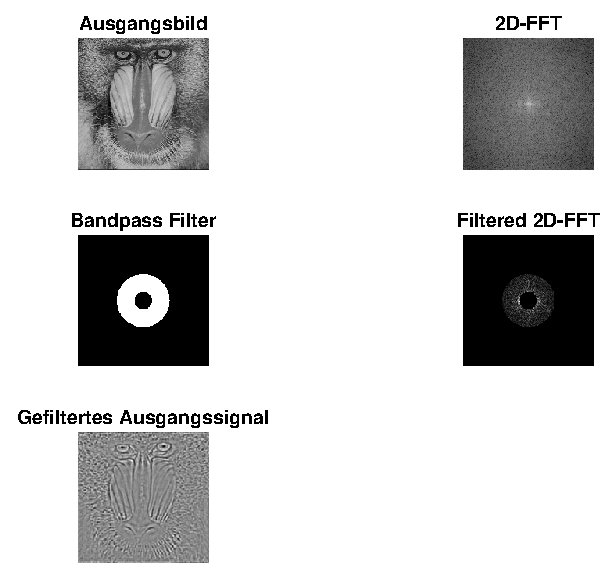
\includegraphics{fig/ex3_1.eps}
        \caption{Edge detection with a bandpass filtered FFT}
        \label{fig:ex3_1}
    \end{figure}
\end{exercise}

\begin{exercise}{FFT in Audio Signal Processing}
    \begin{enumerate}
        \item See Figure \ref{fig:ex4_1}. We can't make any statements about the frequency content of the signal from the plot alone.

              \begin{figure}
                  \centering
                  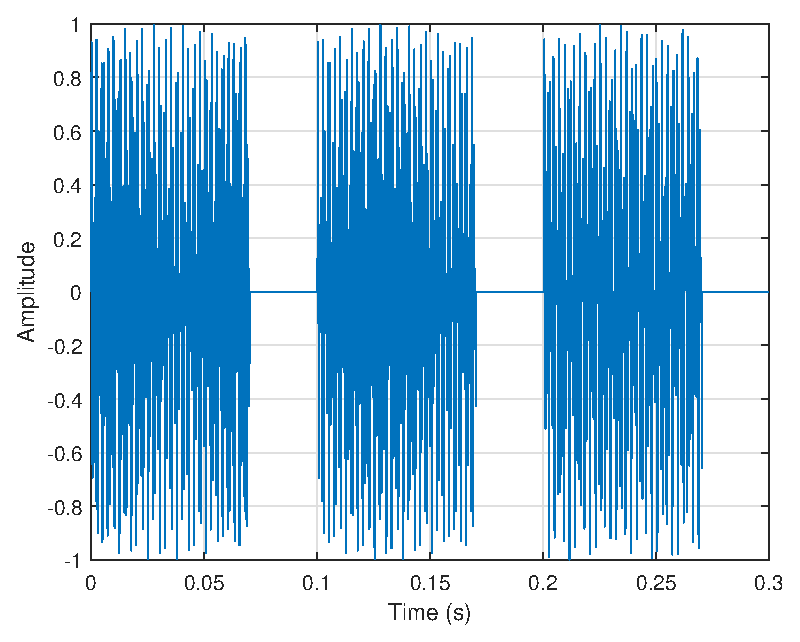
\includegraphics{fig/ex4_1.eps}
                  \caption{First 300 ms of the audio signal}
                  \label{fig:ex4_1}
              \end{figure}

        \item See Figure \ref{fig:ex4_2}.

              \begin{figure}
                  \centering
                  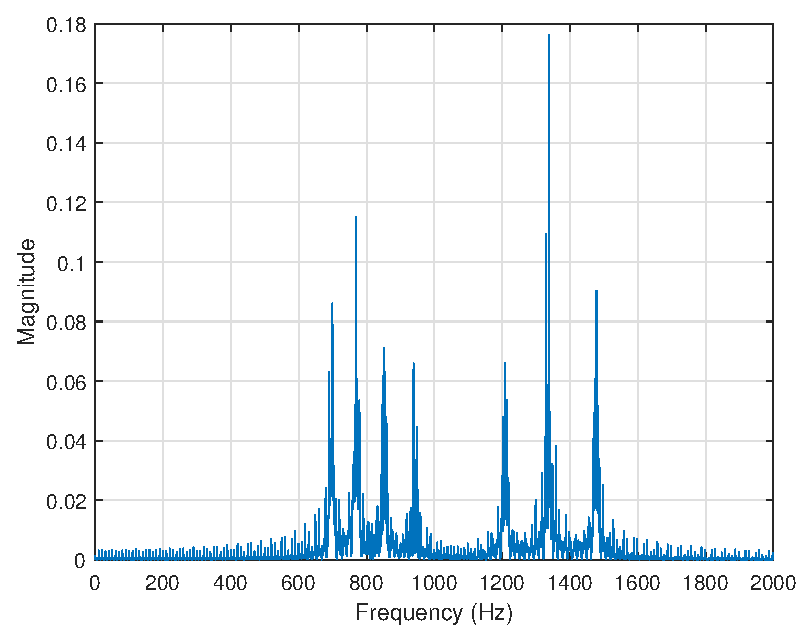
\includegraphics{fig/ex4_2.eps}
                  \caption{FFT of the audio signal (frequencies above 2000 Hz are not shown)}
                  \label{fig:ex4_2}
              \end{figure}

        \item See Figure \ref{fig:ex4_3}.

              \begin{figure}
                  \centering
                  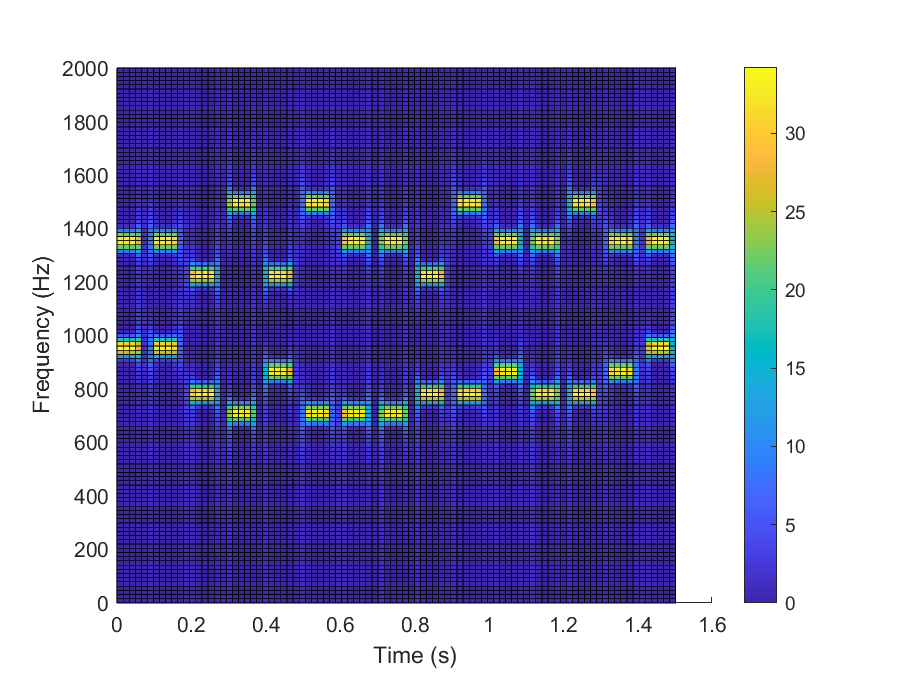
\includegraphics{fig/ex4_3.eps}
                  \caption{Spectrogram of the audio signal with Hamming window.}
                  \label{fig:ex4_3}
              \end{figure}

        \item See Figure \ref{fig:ex4_4}. There is a lot of noise in the plot, compared to the \ref{fig:ex4_3}. This effect is called spectral leakage, which is reduced by the Hamming window (and similar windows).

              \begin{figure}
                  \centering
                  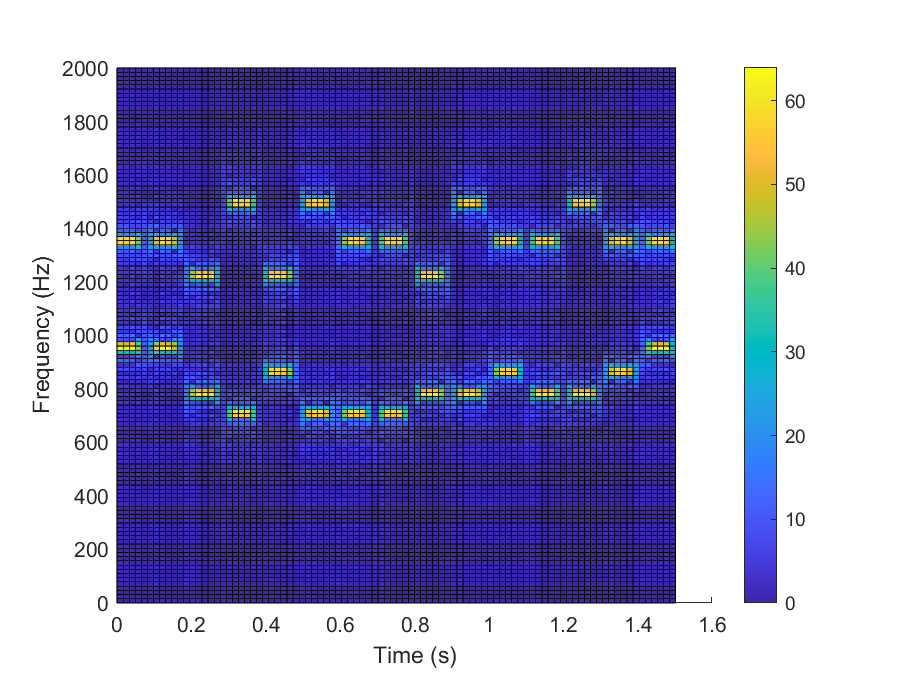
\includegraphics{fig/ex4_4.eps}
                  \caption{Spectrogram of the audio signal without Hamming window.}
                  \label{fig:ex4_4}
              \end{figure}

        \item 0 0 4 3 7 3 2 2 4 6 8 5 6 8 0

        \item
              The spectrogram has time information while the FFT does not. Going just by the FFT, we can't tell when the frequencies (sounds) occur, it might for example be possible that all of them are present at the same time. In the spectrogram we can see that there are alwayes exactly two frequencies present at the same time, and that they change over time, with pauses in between.

              An example of usage could be speech recognition, where the spectrogram can be used to identify the phonemes in the speech signal (since they correspond to frequency bands).
    \end{enumerate}
\end{exercise}

\begin{exercise}{Window effects of the DFT}
    \begin{enumerate}
        \item See Figure \ref{fig:ex5_1}.

              \begin{figure}
                  \centering
                  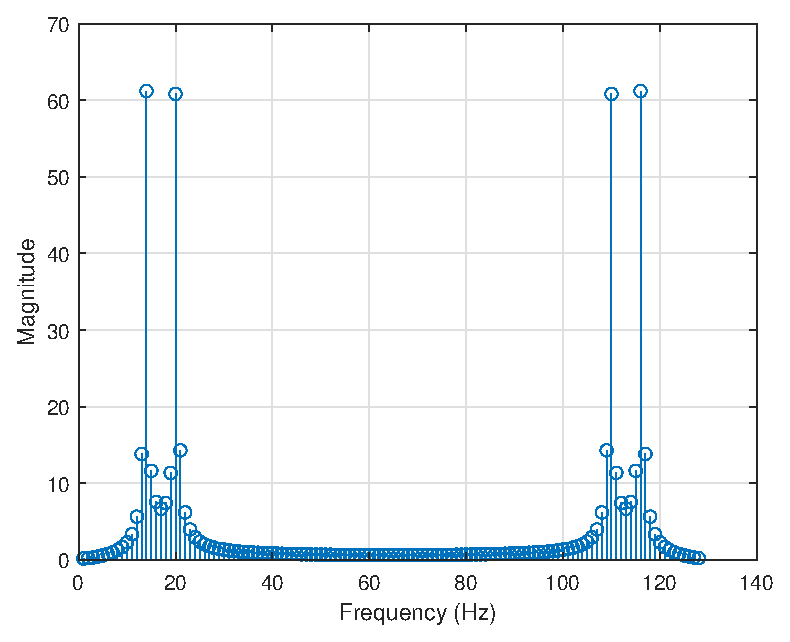
\includegraphics{fig/ex5_1.eps}
                  \caption{DFT of the signal with implicit rectangular window}
                  \label{fig:ex5_1}
              \end{figure}

        \item See Figure \ref{fig:ex5_2}.

              \begin{figure}
                  \centering
                  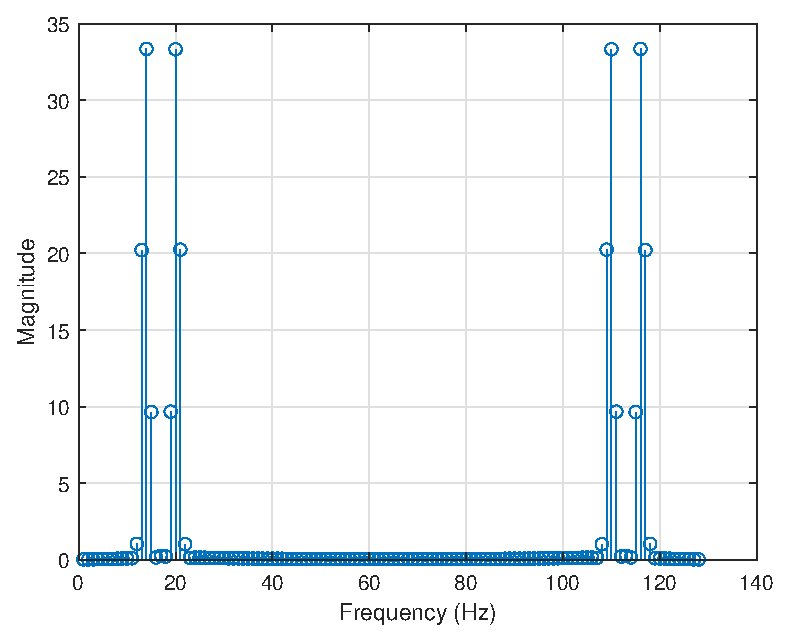
\includegraphics{fig/ex5_2.eps}
                  \caption{DFT of the signal with Hamming window}
                  \label{fig:ex5_2}
              \end{figure}

        \item When using the Hamming window the sidelobes are much lower than in the case of the implicit rectangular window (less spectral leakage). This is unsurprising as it is the main reason to use a smooth window.

        \item TODO
    \end{enumerate}
\end{exercise}

\end{document}
